\documentclass[../main.tex]{subfiles}
\begin{document}

\section{模型建立和求解}
\subsection{模型准备}
% TODO 可以放一个table of contents

% para one
\paragraph{三维热传导方程的推导}
热传导源自温度的不均匀分布,热传导的强弱程度可以用热流强度 \(\vec{q}\),也就是单位时间内通过单位横截面积的热量来进行刻画,温度的不均匀程度可以用温度梯度 \(\nabla u\) 来进行刻画,其中 \(u\) 指的是温度。

傅里叶定律指出,热流强度和温度梯度 \(\nabla u\) 成正比,也就是
\begin{equation}\label{equ:fou}
\vec q = - k \nabla u
\end{equation}
考虑三维空间之中的热量传导,设热源强度,也就是单位时间内在单位体积内部产生的热量为 \(F (x,  y , z, t)\),任取一体积微元 \(\Omega\),应用能量守恒定律有:
\begin{equation}
\oiint _{\, \Omega} \vec q \cdot \mathrm{d} S = \oiiint _{\, \Omega} ( F (x , y , z,t) - u _{t} c \rho ) \, \mathrm{d} V
\end{equation}
其中 \(c\) 是体积微元的比热容,\(\rho\) 为体积微元的密度。

根据散度定理
\begin{equation}
\oiint _{\,\Omega} \vec A  \cdot \mathrm{d} S = \oiiint _{\,\Omega} ( \nabla\kern -1.8pt\vec A) \, \mathrm{d}V
\end{equation}
将其和Equ~(\ref{equ:fou}) 联立可得
\begin{equation}
\nabla \vec q = F (x , y , z ,t) - u_{t} c \rho
\end{equation}
再代入 Equ~(\ref{equ:fou}) 即可得到三维热传导方程:
\begin{equation}\label{equ:cond}
u_{t} c \rho - k\kern 1pt \nabla^{2} u = F (x , y , z, t)
\end{equation}
% TODO 其中 \(k\) 是什么?

% para two
\paragraph{牛顿冷却定律} 牛顿冷却定律指出,两个不同温度的介质之间发生热对流的时候,热流强度和两个介质之间的温度差成正比,也即
\begin{equation}
\vec q = h (u_1 - u_2)
\end{equation}
其中 \(u_1\) 所在的介质指向 \(u_2\) 所在介质的方向向量在 \(\vec q\) 所规定的正方向上具有正分量,将其代入Equ~(\ref{equ:fou}),即得:
\begin{equation}\label{equ:len}
{-k} \nabla u = h ( u_1 - u_2)
\end{equation}
% subsection:模型准备
\subsection{问题1}

% para one
\paragraph{复原间隙温度} 先是复原间隙以及炉前后区域之中的温度,用 \(u\) 表示。

对于两个温区之间的间隙,其只受到两边温区的加热,并且间隙之中并没有热源,三维热传导方程Equ~(\ref{equ:cond})中 \(F ( x , y , z ,t) = 0\),且退化为一维热传导方程:
\begin{equation}
\frac{\partial u}{\partial t} = a^{2} \frac{\partial ^{2} u}{ \partial x ^{2}}
\end{equation}
% TODO 在这里 \(a\) 是什么?
考虑到温度已经稳定,也就是温度不再变化,也就是 \(\frac{\partial u}{ \partial t} = 0\), 于是有 \(\frac{\partial ^{2} u}{\partial x ^{2}} = 0 \),
也即,间隙中的温度关于 \(x\) 是线性变化的。于是说给定了两边温区的温度之后,假设是 \((x_1, T_1), (x_2, T_2)\), 就能够得出间隙中的温度关于距离 \(x\) 的表达式:
\[
u(x)  = T_{1} + \frac{T_2 - T_1}{x_2 - x_1} \cdot x
\]
能够根据温区的温度给出炉内上下表面的温度曲线。对于附件所描述的某次实验,\(T _{1 \sim 5} = 17 5 ^{\circ}\mathrm{C}\), \(T _{6} = 195 ^{\circ}\mathrm{C}\), \(T _{7} = 235 ^{\circ}\mathrm{C}\), \(T _{8 \sim 9} = 255 ^{\circ}\mathrm{C}\),以炉前区域最左端为\(x\)起点,能够得到温度 \(u\) 关于距离 \(x\) 的函数图像,见图~\ref{fig:1},温度 \(u\) 关于距离 \(x\) 的函数记为 \(u ^{\dagger}\)。
\input pic.tex

% para
\paragraph{温度分布方程的导出}
不妨设炉内的温度分布为 \(u ( x,  y  ,z ,t)\),由于炉内的温度沿着 \(z\) 轴对称分布,因此为 \(\frac{\partial u}{ \partial z} = 0\)。由题意,回焊炉启动之后,颅内空气温度会在短时间内达到稳定,因此 \( \frac{\partial u}{ \partial t} = 0\)。代入三维热传导方程Equ~(\ref{equ:cond})得:
\begin{equation}
0 - k \bigg( \frac{\partial ^{2} u }{\partial x ^{2}} + \frac{\partial ^{2} u}{\partial x ^{2}} + 0\bigg) = F (x , y, z , t)
\end{equation}
又由于考察的区域为不包含温区的传动带区域,因此 \(F (x, y , z , t) = 0\),故上式转化为:
\begin{equation}
\frac{\partial ^{2} u}{\partial x ^{2}} + \frac{\partial ^{2} u}{\partial y ^{2}} = 0
\end{equation}
能够知道 \(u\) 只是 \(x , y\) 两个维度的函数,且满足拉普拉斯方程。

由于 \(u\) 不是关于 \(t\) 的函数,故不必考虑方程的初始条件
考察温区间隙的温度分布 \(u (x,  y , z ,t)\)。根据模型假设,温区间隙的热流仅沿 \(x\) 轴方向传播,则对于间隙有,\(\frac{\partial u}{\partial y} = 0\)。与炉内同理,\(\frac{\partial u}{ \partial z} = 0\),\(\frac{\partial u}{\partial t} = 0\),\(F(x, y , z,t) = 0\)。可知\(u\)仅为 \(x\) 的函数。代入三维热传导方程 Equ~(\ref{equ:cond}),有:
\begin{equation}
0 - k \bigg( \frac{\partial ^{2} u}{ \partial x ^{2}} + 0 + 0\bigg) = 0
\end{equation}
也就是 
\begin{equation}
\frac{\partial ^{2} u}{\partial x ^{2}} = 0
\end{equation}
由于 \(u\) 是关于 \(x\) 的函数,可知 \(u = kx + b\),即温度为 \(u_{1} , u_2\) 的两个温区的间隙的温度分布为 \(u = \displaystyle \frac{u_2 - u_1}{\varDelta d} ( x - x_1) + u_1\),其中 \(\varDelta d\) 是间隙的长度。

于是,视炉前区域、炉后区域为第\(0\), 12 个小温区,假设第\(i\)个小温区的温度为 \(u_{i}\),左右两侧作坐标为 \(x_{il}\), \(x_{ir}\),并且假设上下两个温区之间间距为 \(l\),炉前区域、炉后区域之间间距为 \(l_{0}\),则炉内温度分布的边界条件为
\begin{equation}
\begin{cases}
u|_{y = \pm l/2} = 
\begin{cases}
\frac{u_{i+1} - u_{i}}{\varDelta d} (x - x_{ir}) + u_{i} , & \quad x _{ir} < x < x_{i+1 l} \\
u_{i} = 25 ^{\circ}\mathrm{C}, & \quad  x_{il} \le x \le x_{ir} 
\end{cases} \\
u|_{x = 0} = 25 ^{\circ}\mathrm{C}\\
u|_{x = l_{0}} =  25 ^{\circ}\mathrm{C}
\end{cases}
\end{equation}
综上,回焊炉内部的温度分布方程为
\begin{equation}
\begin{cases}
\displaystyle\frac{\partial ^{2} u}{\partial x ^2} + \frac{\partial ^{2} u}{\partial y ^{2}} = 0\\
u|_{y = \pm l/2} = 
\begin{cases}
\displaystyle\frac{u_{i+1} - u_{i}}{\varDelta d} (x - x_{ir}) + u_{i} , & \quad x _{ir} < x < x_{i+1 l} \\
\displaystyle u_{i} = 25 ^{\circ}\mathrm{C}, & \quad  x_{il} \le x \le x_{ir} 
\end{cases} \\
u|_{x = 0} = 25 ^{\circ}\mathrm{C}\\
u|_{x = l_{0}} =  25 ^{\circ}\mathrm{C}
\end{cases}
\end{equation}
% TODO 这一部分和 par one 重复

%%
\paragraph{拉普拉斯方程的数值求解} 根据逐次超松弛迭代法,使用网格化分割方法,可以列出如下迭代方程
\begin{equation}
u_{k,j} ^{(i)} = \frac{\beta}{4} \bigg( u_{k-1, j} ^{(i)} + u_{k,j-1} ^{(i)} + u_{k+1,j} ^{(i-1)}+ u _{k, j+ 1} ^{(i-1)} \bigg) + (1- \beta) u_{k,j} ^{i-1} ,\quad \beta \in (1, 2]
\end{equation}
其中 \(i\) 为迭代次数,可以绘制出下面 \(u ( x , y)\) 图像

\begin{figure}[H]
\centering
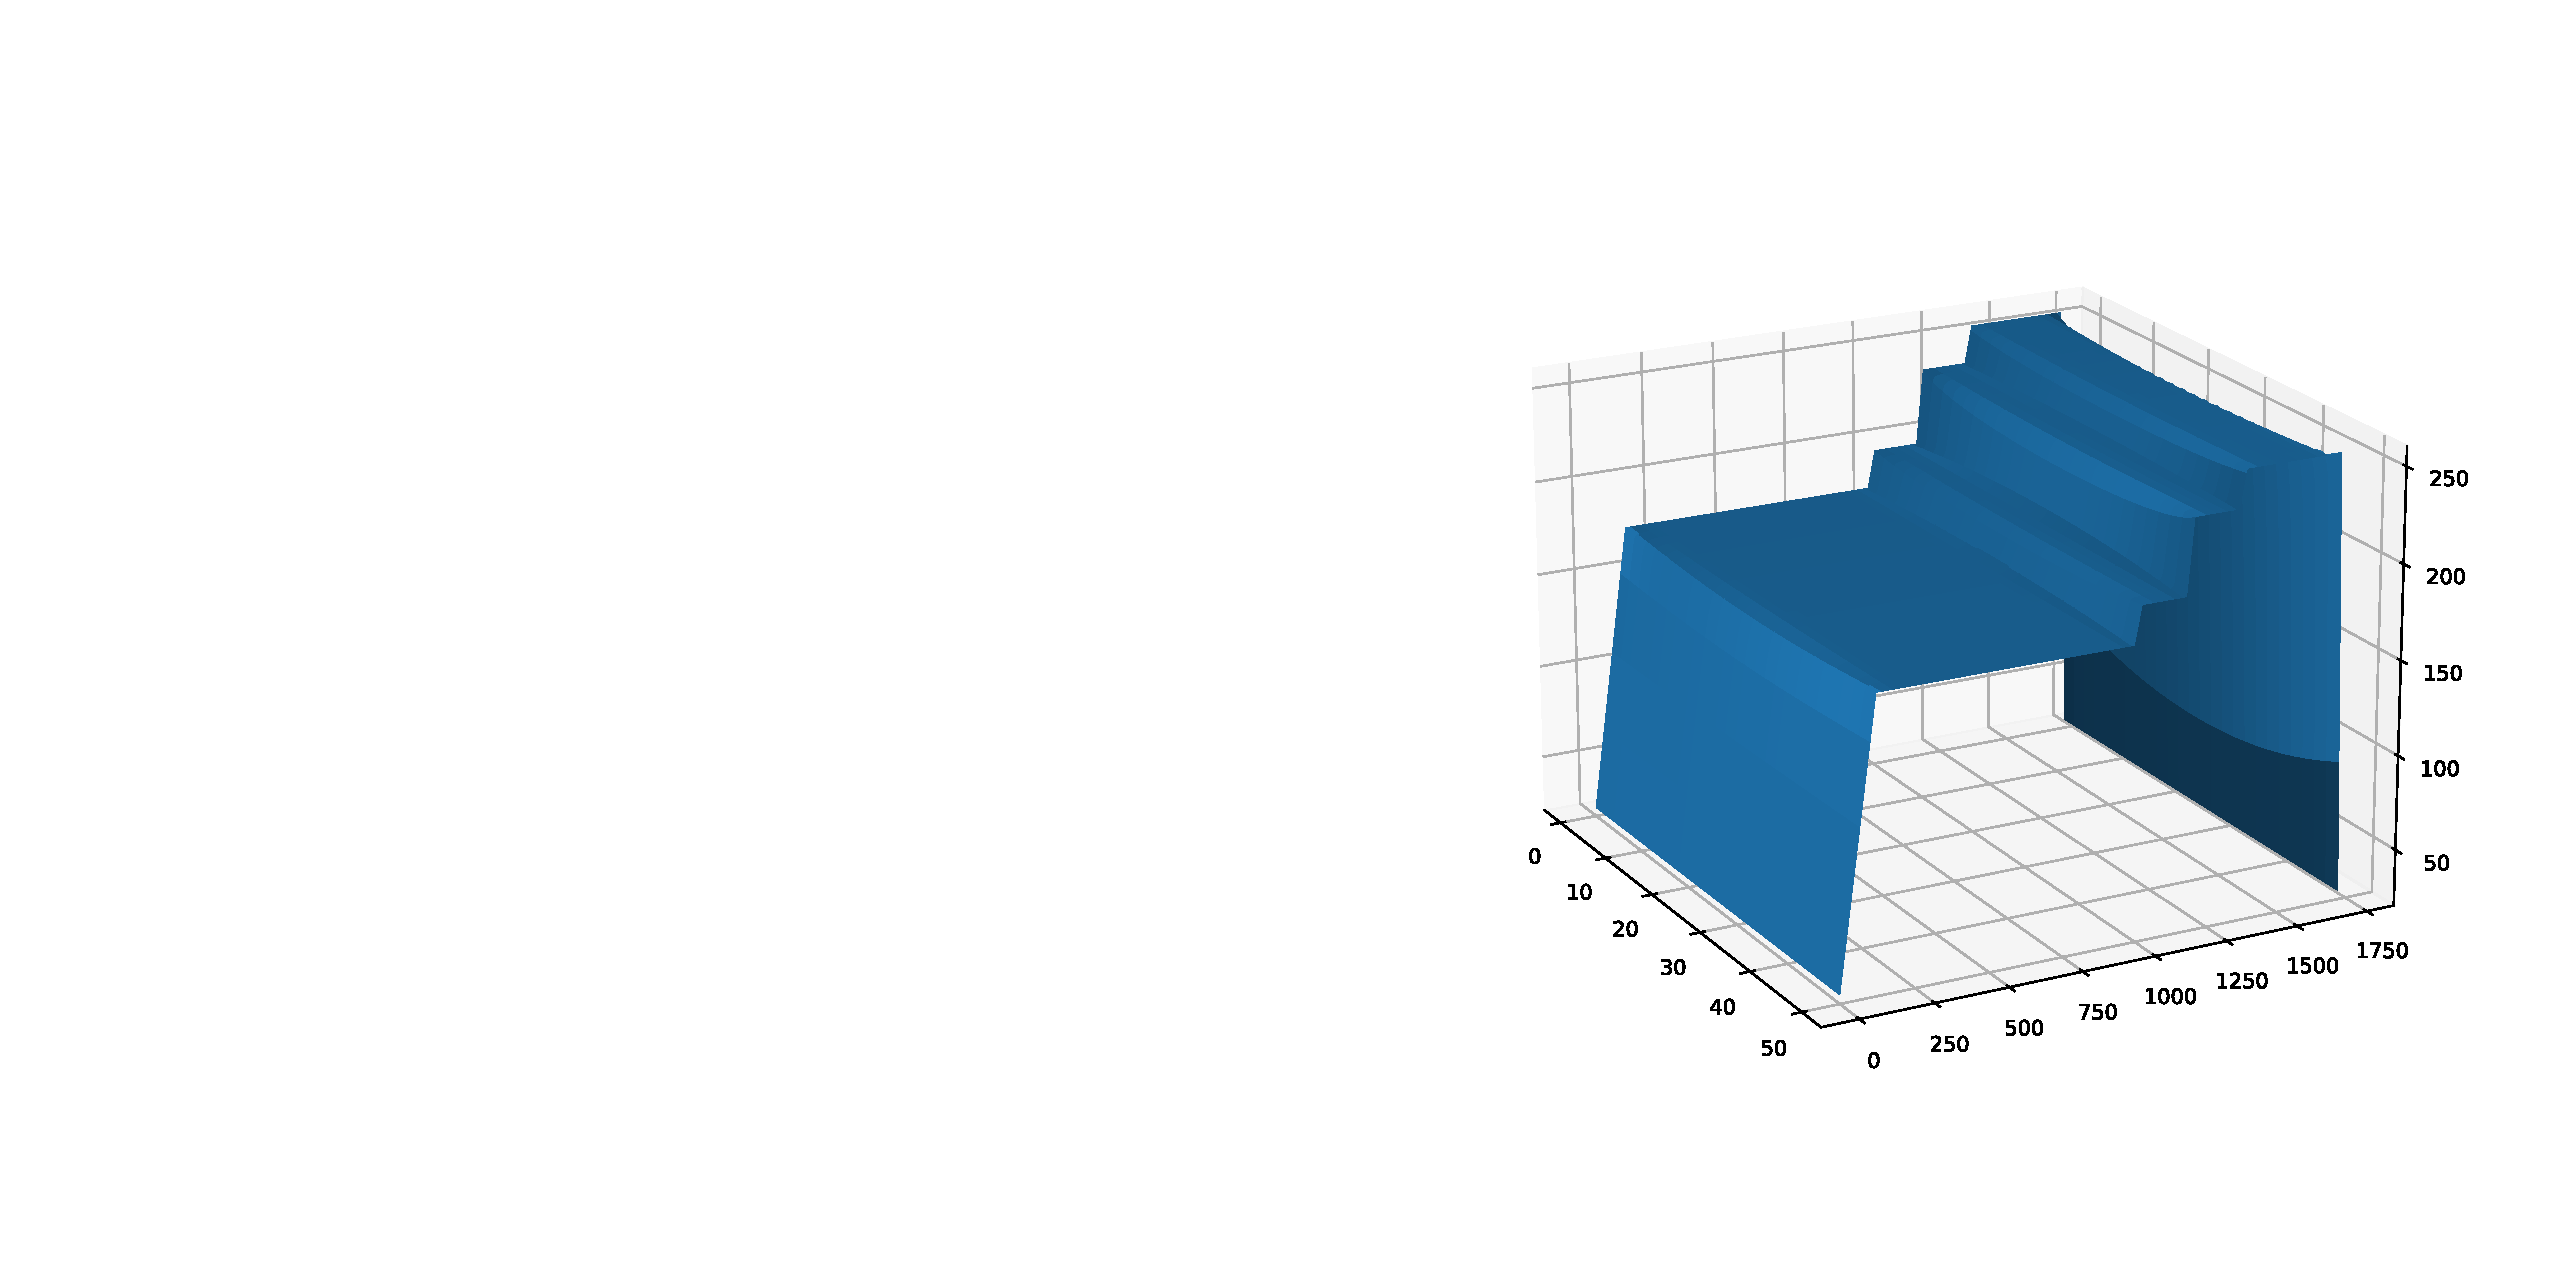
\includegraphics[scale = 0.5]{fig1.pdf}\caption{什么图像}
\end{figure}
% TODO


%%
\paragraph{确定热传导方程} 对于中间部分的焊接材料,设其在受到加热的时候温度为 \(v\),热传导率为 \(k\),密度为 \(\rho\),比热容为 \(c\),此时空气和焊锡之间的热对流系数为 \(h\),于是三维热传导方程Equ~(\ref{equ:cond})之中的 \(F (x, y , z, t)\) 满足 \(F ( x , y , z ,t ) = 0\),由于焊接材料只在厚度这一个方向上传热,于是三维热传导方程退化为在 \(y\) 轴方向上传热的热传导方程,也即
\begin{equation}\label{equ:one-dim}
\frac{\partial v}{\partial t} - a ^{2} \frac{\partial^{2} v }{\partial y ^{2}} = 0
\end{equation}
% TODO 其中 \(a\) 是?

初始时,其温度为车间温度,也即,当时刻为零的时候,\(v\) 的值为 \(25 ^{\circ}\mathrm{C}\)。
\begin{equation}
v (y, 0) = 25 ^{\circ}\mathrm{C}, \quad y \in [0, {\it height}\kern 1pt]
\end{equation}
在这里将 \(v\) 视为两个参数的函数,接收 \(y\) 轴方向上的坐标\(y\)以及时间 \(t\)。

由于焊接材料仅在 \(y\) 轴一个方向上传热,傅里叶热传导方程 Equ~\ref{equ:fou} 可以退化为
\begin{equation}
\vec q = {-} k \frac{\partial v}{ \partial y}
\end{equation}
将 \(\vec q\) 代入牛顿冷却定律Equ~\ref{equ:len},并对焊接材料两端和空气之间的热对流过程进行分析,可得边界条件:
\begin{equation}\label{equ:bian}
\begin{cases}
\displaystyle- k \left.\frac{\partial v}{\partial y}\right|_{y = 0} =  h \Big[ u(t) - v(0, t)\Big] \\
\displaystyle- k \left.\frac{\partial v}{\partial y}\right|_{y = {\it height}} = h \Big[v({\it height}, t) - u(t)\Big]
\end{cases}
\end{equation}
其中\(u(t)\) 是对应时刻,焊接材料表面的空气温度。\(u ^{\dagger}\) 为温度关于距离 \(x\) 的函数,在上文之中已经求出,则 \(u (t) = u^{\dagger} ( Vt)\),其中 \(V\) 是过炉速度。
综上,可对热传导模型建立如下方程:
\begin{equation}
\begin{cases}
\displaystyle \frac{\partial v}{\partial t} - a ^{2}  \frac{\partial ^{2} v}{\partial y^{2}} = 0 \\
\displaystyle v (y , 0) = 25 ^{\circ}\mathrm{C}, \quad y \in [0, {\it height\kern 1pt}] \\
\displaystyle- k \left.\frac{\partial v}{\partial y}\right|_{y = 0} =  h \big[u(t) - v(0, t)\big] \\
\displaystyle- k \left.\frac{\partial v}{\partial y}\right|_{y = {\it height}} = h \big[v({\it height}, t) - u(t)\big]
\end{cases}
\end{equation}

%%
\paragraph{差分形式}
将边界条件差分化,对于任意时刻,有
\begin{equation}
\begin{cases}
\displaystyle - H \cdot \frac{v _{1, t}  - v _{0, t}}{\mathrm{dy}} + v_{0 ,t} = u_{t} \\
\\
\displaystyle H \cdot\frac{v_{M , t} - v _{M-1, t}}{\mathrm{dy}} + v_{M,t} = u_{t}
\end{cases}
\end{equation}
其中 \(H = \dfrac{k}{h}\),\(\mathrm{dy}\) 是距离步长,\(v_{i,j}\) 是焊接材料温度 \(v\) 离散化后的结果,\(i\) 为距离指标 \(i = 0,  1,  2 , \dots , M\), \(j\) 是时间指标 \(j = 0 , 1 , 2 , \dots, N\)。对上式子进行化简能够得到:
\begin{equation}
\begin{cases}
\displaystyle v_{0,t} = \frac{H}{H + \mathrm{dy}} v_{1 ,t} + \frac{\mathrm{dy}}{H + \mathrm{dy}} \cdot u_{t}\\
\\
\displaystyle v_{M,t} = \frac{H}{H + \mathrm{dy}} v _{M-1, t} + \frac{\mathrm{dy}}{H + \mathrm{dy}} \cdot u_{t}
\end{cases}
\end{equation}
而对于焊接材料的一维热传导方程 Equ~(\ref{equ:one-dim})进行差分化,能够得到一个半差分形式:
\begin{equation}
\frac{\partial v _{i}}{\partial t} = a \cdot \frac{u_{i+1, t} - 2 u_{i, t} + u_{i- 1 , t}}{\mathrm{dy} ^{2}}
\end{equation}
在这里时间差分采用向后欧拉法,得到全差分格式如下:
\begin{equation}\label{equ:all}
\frac{\mathbf{v}_{t+1}  - \mathbf{v}_{t}}{\tau}= \frac{a}{\mathrm{dy}^{2}} (\mathbf{A}\mathbf{v} _{t+1} + \mathbf{b})
\end{equation}
其中 \(\tau\) 是时间步长,\(\mathbf{v}_{t}\) 是一个向量,其值为 \([v _{1, t}, v_{2, t}, \dots, v_{M, t}]^{\mathrm{T}}\),也即,时间指标为 \(t\) 的时候焊接材料上面各个点温度所组成的向量,其中矩阵\(\mathbf A\) 满足
\begin{equation}
\mathbf{A} = 
\begin{bmatrix}
\frac{H}{H + \mathrm{dy}} - 2 & 1 &&\\
\\[-10pt]
1 & -2 & 1 &\\
& & 1 & -2 & 1 \\
\hdotsfor{6}\\
\\[-10pt]
&& & 1 & -2 & 1 \\
\\[-10pt]
&& &  & 1 &\frac{H}{H + \mathrm{dy}} -2 
\end{bmatrix}
\end{equation}
并且 \(\mathbf{b} = \displaystyle \bigg[ \frac{\mathrm{dy}}{H + \mathrm{dy}} \cdot u_{t} , 0 ,\dots, 0 , \frac{\mathrm{dy}}{H + \mathrm{dy}} \cdot u_{t} \bigg] ^{\mathrm{T}}\)。
令 \(r = \displaystyle \frac{a \tau}{h ^{2}}\),随后根据全差分形式~\ref{equ:all},化简得到
\begin{equation}\label{equ:iter}
(\mathbf{I} - r\mathbf{A} ) \mathbf{v} _{t+1} = \mathbf{v}_{t} + r \mathbf{b}
\end{equation}
本文使用迭代形式 Equ~(\ref{equ:iter}) 进行 \(\mathbf{v}_{t}\) 的迭代。

对于 \(\mathbf{I} - r \mathbf{A}\),其值为
\begin{equation}
\mathbf{I} - r \mathbf{A} =
\begin{bmatrix}
1 - \big(\frac{H}{H + \mathrm{dy}}\big) r & -r \\
-r & 1 + 2r & -r \\
\hdotsfor{5}\\
&&-r & 1 + 2r & -r \\
&&& -r & 1 - \big(\frac{H}{H + \mathrm{dy}}- 2\big)r
\end{bmatrix}
\end{equation}

%% par
\paragraph{分段拟合} 考虑到焊接材料的性质会根据材料本身的温度发生改变,在不同区域内部焊接材料的热扩散系数\(A\)和焊接材料和空气之间的热对流交换系数\(h\)也不同,本文将整个加热过程分为三段,假设每一段之中热扩散系数和热对流交换系数不发生改变,这三段的系数表示为 \(A_{i}, h_{i}\), \(i = 1 , 2 ,3 \),并进行分段拟合求出 \(A_{i} ,h_{i}\)。

本文将加热过程按照炉温的高低分为三段:低温区、高温区和冷却区:
\begin{table}[H]
\centering
\begin{tabular}{ccc}
编号&区域 & 范围 / cm \\ \hline \hline
\\ [-1em]
I&低温区& \([0 , 200]\) \\
II&高温区& \([200, 342]\) \\
III&冷却区& \([342, 435.5]\) 
\\ [-1em]
\\ \hline
\end{tabular}\caption{根据炉温划分的区域}
\end{table}
低温区是炉前区域的最左端到第五个小温区和第六个小温区之间的间隙的中点,高温区是低温区末端到第九个小温区和第十个小温区之间的间隙的中点,剩余部分便是冷却区。

本文先是对低温区域进行拟合,得出低温区的焊接材料的参数,也就是 \(A_{1}, h_{1}\)。得到的低温区域末端的温度作为高温区的初始条件,同样进行拟合,得到高温区的焊接材料的参数 \(A_{2}, h_{2}\)。同理得到 \(A_{3}, h_{3}\)。拟合得到的结果如下表
\begin{table}[H]
\centering
\begin{tabular}{ccc}
& \(A_{i}\) \(\mathrm{W}/ (\mathrm{m}\cdot \mathrm{K})\) & \(h_{i}\) \(\mathrm{W} / (\mathrm{m}^{2} \cdot \mathrm{K})\) \\ \hline \hline
\\[-1em]
I & \(5 \times 10 ^{-11}\) & \(5 \times 10 ^{-6}\) \\ 
II & \(6 \times 10 ^{-11}\) & \(4 \times 10 ^{-7}\) \\
III & \(3 \times 10 ^{-11}\) & \(1 \times 10 ^{-5}\) 
\\[-1em]
\\ \hline
\end{tabular}\caption{焊接材料在不同区域内拟合出的参数}
\end{table}

\subsection{问题2}
根据题意,找到的最大的过炉速度 \(V\) 需要满足下面条件,焊接材料的中心位置的温度 \(v\)是关于时间\(t\)的函数,有:

\begin{table}[H]
\centering
\begin{tabular}{ccccc}
编号&限制 & min & max 	& 单位
\\ [-1em]
\\ \hline \hline
\\ [-1em]
1&\(\vert v '\vert\) & 0 & 3 & \(^{\circ}\mathrm{C} / \mathrm{s}\)\\
2&处于 \(150 ^{\circ}\mathrm{C}\sim 190 ^{\circ}\mathrm{C}\) 的时间 & 60 & 120 & \(\mathrm{s}\)\\
3&大于 \(217 ^{\circ}\mathrm{C}\) 的时间 & 40 & 90 & \(\mathrm{s}\)\\
4&\(\max {v}\) & 240 & 250 & \(^{\circ}\mathrm{C}\) 
\\ [-1em]
\\ \hline
\end{tabular}
\end{table}
为了使用二分搜索进行边界值的查找,需要验证上面四个限制条件能够使用二分法。
\begin{enumerate}
\item 
对于焊接材料两边的表面的空气温度 \(u\),其能够写为关于时间 \(t\) 的函数:
\[
u (t) = u^{\dagger} ( Vt)
\]
在这里 \(u ^{\dagger}\) 炉内温度关于与炉前区域最左侧的距离的函数,\(V\) 是过炉速度。于是有:
\begin{equation}
\frac{\mathrm{d} u}{\mathrm{d} t} = V \frac{\mathrm{d} u ^{\dagger}}{\mathrm{d} x}
\end{equation}
根据问题一之中已经求出的炉内空气在焊接材料所在的中心线上的温度曲线,在低温区以及高温区之中,\(\mathrm{d} u ^{\dagger}/ \mathrm{d} x\) 的值始终大于等于\(0\)。于是根据上式,在某一个时刻,\(V\) 越大则 \(\mathrm{d} u / \mathrm{d} t\) 越大。根据边界条件 Equ~\ref{equ:bian},在低温区或者是高温区内部焊接材料的温度变化率 \(\vert v' \vert\)和其所在的炉内的空气温度成正相关。于是得出焊接材料的温度变化率 \(\vert v'\vert\)是和过炉速度 \(V\)成正相关的,过炉速度越快,温度的变化速率就越快。那么对于限制条件 1 对应的边界值,能够使用二分搜索进行查找。

\item 
作为上述结论的推论,\(v\) 处于 \(150 ^{\circ}\mathrm{C}\sim 190 ^{\circ}\mathrm{C}\) 的时间,和过炉速度成负相关,左边界值和右边界值都能使用二分搜索进行查找。

\item 
若使焊接材料的温度大于 \(217 ^{\circ}\mathrm{C}\),其周边的空气温度应当大于 \(217 ^{\circ}\mathrm{C}\),根据温区表面的温度曲线~\ref{fig:1},得知,焊接材料
% TODO
\item
对于限制条件 4 
% TODO
\end{enumerate}

\subsection{问题 3}
针对问题3中最优炉温曲线的求解,易知是一个多元连续函数优化问题。小温区1~5、小温区6、小温区7、小温区8~9这四个决策变量分别对应着四个取值区间\([165 ^{\circ}\mathrm{C}, 185^{\circ}\mathrm{C}]\)\([185 ^{\circ}\mathrm{C}, 205 ^{\circ}\mathrm{C}]\), \([225 ^{\circ}\mathrm{C}, 245 ^{\circ}\mathrm{C}]\), \([245 ^{\circ}\mathrm{C} , 265 ^{\circ}\mathrm{C}]\),根据目标函数()以及最终的优化目标,即理想的炉温曲线应使超过\(217 ^{\circ}\mathrm{C}\)到峰值温度所覆盖的面积最小,本文拟采取十进制蚁群算法,对各温区温度进行搜索。

以下本文将以一元连续函数为例,说明十进制蚁群算法的原理。设一元连续函数优化的数学模型如下:
\begin{equation}
\min f(x), \quad x \in [x_1 , x_2]
\end{equation}
\end{document}
